%%% Local Variables:
%%% coding: utf-8
%%% mode: latex
%%% TeX-engine: xetex --shell-escape
%%% End:

\documentclass[14pt, a4paper]{extarticle}

\usepackage{graphicx}
\DeclareGraphicsExtensions{.jpg,.png}

\usepackage{hyperref}

\usepackage{amsfonts}
\usepackage{amsmath}

\usepackage[english,russian]{babel}

\usepackage{fontspec} 
\defaultfontfeatures{Ligatures={TeX},Renderer=Basic}
\setmainfont[Ligatures={TeX,Historic}]{Times New Roman}
\setmonofont{Courier New}
\newfontfamily\cyrillicfonttt[Script=Cyrillic]{Courier New}
\urlstyle{same}

\usepackage{xcolor}

\usepackage{tabularx}

\usepackage{indentfirst} %отступ первой строки первого абзаца
\linespread{1.25}

\usepackage{geometry}
\geometry{left=3cm}
\geometry{right=1cm}
\geometry{top=2cm}
\geometry{bottom=2cm}

\hypersetup{
    colorlinks,
    citecolor=black,
    filecolor=black,
    linkcolor=black,
    urlcolor=black
}

\usepackage[final]{pdfpages}

\usepackage{titlesec} % оформление заголовков

\titleformat{\section}[block]
	{\newpage\hspace{\parindent}\bfseries\fontsize{18pt}{21.6pt}\selectfont}
        {\thesection}
        {1em}{\MakeUppercase}
\titleformat{name=\section,numberless}[block]
	{\newpage\centering\bfseries\fontsize{18pt}{21.6pt}\selectfont}
        {}
        {1em}{}
\titleformat{\subsection}[block]
	{\bfseries\hspace{\parindent}\fontsize{16pt}{19.2pt}\selectfont}
        {\thesubsection}
        {1em}{}
        
\usepackage{float}
\usepackage{caption}

\usepackage[newfloat]{minted}
\newenvironment{code}{\captionsetup{type=listing}}{}
\SetupFloatingEnvironment{listing}{name=Листинг}
\usepackage{fancyvrb}

\DeclareCaptionLabelSeparator{emdash}{\;\textemdash\;}
\captionsetup[figure]{name={Рисунок}, labelsep=emdash, justification=centering, singlelinecheck=off, font={small, bf}, labelfont=bf}
\captionsetup[table]{name={Таблица}, labelsep=emdash, justification=raggedright, singlelinecheck=off, font={small, it}, labelfont=it}
\captionsetup[listing]{name={Листинг}, labelsep=emdash, justification=raggedright, singlelinecheck=off, font={small, it}, labelfont=it}

\usepackage{array}
\newcommand\ChangeRT[1]{\noalign{\hrule height #1}}

\usepackage{ragged2e}
\usepackage{microtype}

\justifying
\sloppy
\tolerance=500
\hyphenpenalty=10000
\emergencystretch=3em

\usepackage{setspace}

\begin{document}

\makeatletter
\renewcommand{\l@section}{\@dottedtocline{1}{0em}{1.25em}}
\renewcommand{\l@subsection}{\@dottedtocline{2}{0em}{1.75em}}
\renewcommand{\l@subsubsection}{\@dottedtocline{3}{0em}{2.6em}}
\renewcommand{\@dotsep}{1.25}
\makeatother

\def\contentsname{СОДЕРЖАНИЕ}

%\pagenumbering{gobble}
\begin{titlepage}

\includepdf{title}
\end{titlepage}
%\tableofcontents

\section*{Теоритическое введение}
Класс FileWriter является производным от класса Writer. Он
используется для записи текстовых файлов.

Чтобы создать объект FileWriter, можно использовать один из
следующих конструкторов:
\begin{itemize}
\item FileWriter(File file);
\item FileWriter(File file, boolean append);
\item FileWriter(FileDescriptor fd);
\item FileWriter(String fileName);
\item FileWriter(String fileName, boolean append);
\end{itemize}

Так, в конструктор передается либо путь к файлу в виде строки,
либо объект File, который ссылается на конкретный текстовый файл.
Параметр append указывает, должны ли данные дозаписываться в конец
файла (если параметр равен true), либо файл должен перезаписываться.

В конструкторе использовался параметр append со значением false
- то есть файл будет перезаписываться. Затем с помощью методов,
определенных в базовом классе Writer производится запись данных.

Класс FileReader наследуется от абстрактного класса Reader и
предоставляет функциональность для чтения текстовых файлов.

Для создания объекта FileReader мы можем использовать один из
его конструкторов:
\begin{itemize}
\item FileReader(String fileName);
\item FileReader(File file);
\item FileReader(FileDescriptor fd);
\end{itemize}
\section*{Постановка задачи}
Реализовать запись в файл введённой с клавиатуры информации.
\section*{Программный код}
\begin{code}
\captionof{listing}{Основной код}
\inputminted[frame=single, fontsize=\footnotesize]{java}{Main.java}
\end{code}
\section*{Вывод программы}
\begin{figure}[H]
\centering
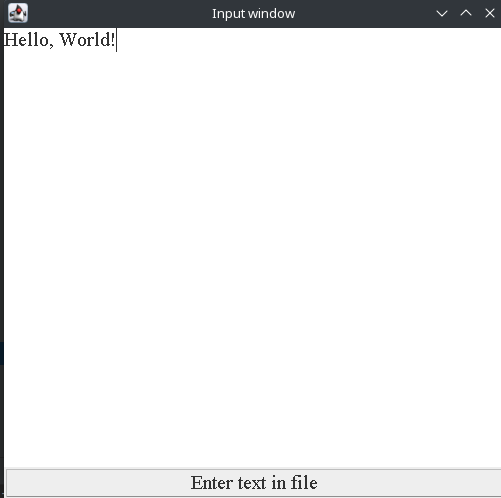
\includegraphics[scale=0.5]{output}
\caption{Ввод через графический интерфейс}
\end{figure}
\begin{figure}[H]
\centering
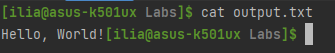
\includegraphics[scale=1]{terminal}
\caption{Данные файла output.txt}
\end{figure}
\section*{Вывод}
В ходе данной лабораторной работы были освоены на практике работа с файлами на языке Java. Получены практические навыки по чтению и записи данных в файл.
\end{document}